% !TeX root = ../main.tex

\section{Automazione del Processo di Sviluppo}

\begin{frame}{Processo di Sviluppo}

    \begin{figure}[H]
        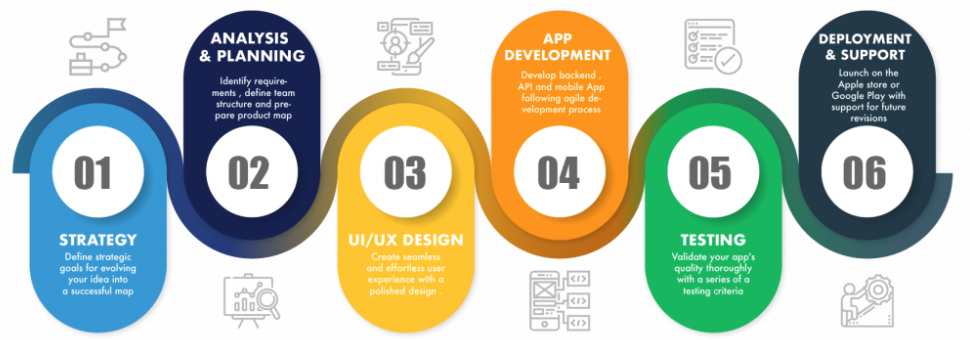
\includegraphics[width=1\textwidth]{img/sdlc2.png}
    \end{figure}

\end{frame}

\begin{frame}{Pratiche DevOps}
    \begin{columns}[onlytextwidth,t]
        \begin{column}{0.45\textwidth}
    
            \textbf{Continuous Integration}
            \vspace{2mm}
            \begin{itemize}
                \item \textbf{Principio}: Integrazione frequente di piccole modifiche, testate automaticamente
                \vspace{2mm}
                \item \textbf{Stages}:
                \begin{itemize}
                    \item Build
                    \item Test
                    \item Package
                \end{itemize}
            \end{itemize}
            
        \end{column}
        \begin{column}{0.45\textwidth}

            \textbf{Continuous Delivery}:
            \vspace{2mm}
            \begin{itemize}
                \item \textbf{Principio}: Rilascio frequente di piccole modifiche, eseguito in modo automatico
                \vspace{2mm}
                \item \textbf{Stages}:
                \begin{itemize}
                    \item Release alpha
                    \item Release beta
                    \item Release prod
                \end{itemize}
            \end{itemize}
        
        \end{column}
    \end{columns}

    \vspace{2mm}

    \begin{figure}[H]
        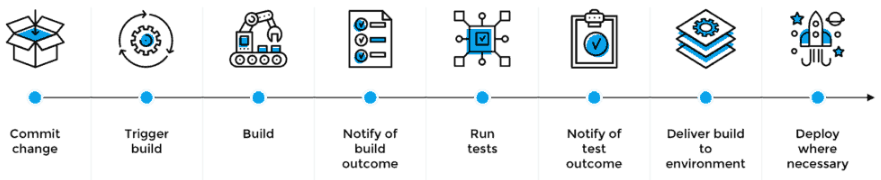
\includegraphics[width=0.9\textwidth]{img/cicd.png}
    \end{figure}

\end{frame}

\begin{frame}{Flusso di Lavoro}
    \begin{figure}[H]
        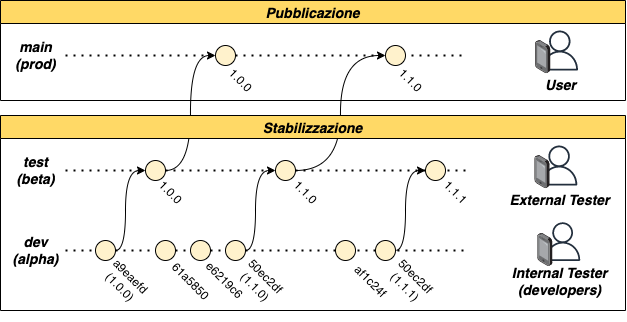
\includegraphics[width=0.8\textwidth]{img/release-flow.png}
    \end{figure}

    \textbf{Caratteristiche}:
    \begin{itemize}
        \item 3 branch principali (dev, test, main)
        \item 3 ``ambienti'' associati (alpha, beta, prod)
        \item Riutilizzabile (Template)
        \item Estendibile (Pipeline-as-Code)
    \end{itemize}
\end{frame}

\begin{frame}{Sistema Complessivo}

    \begin{figure}[H]
        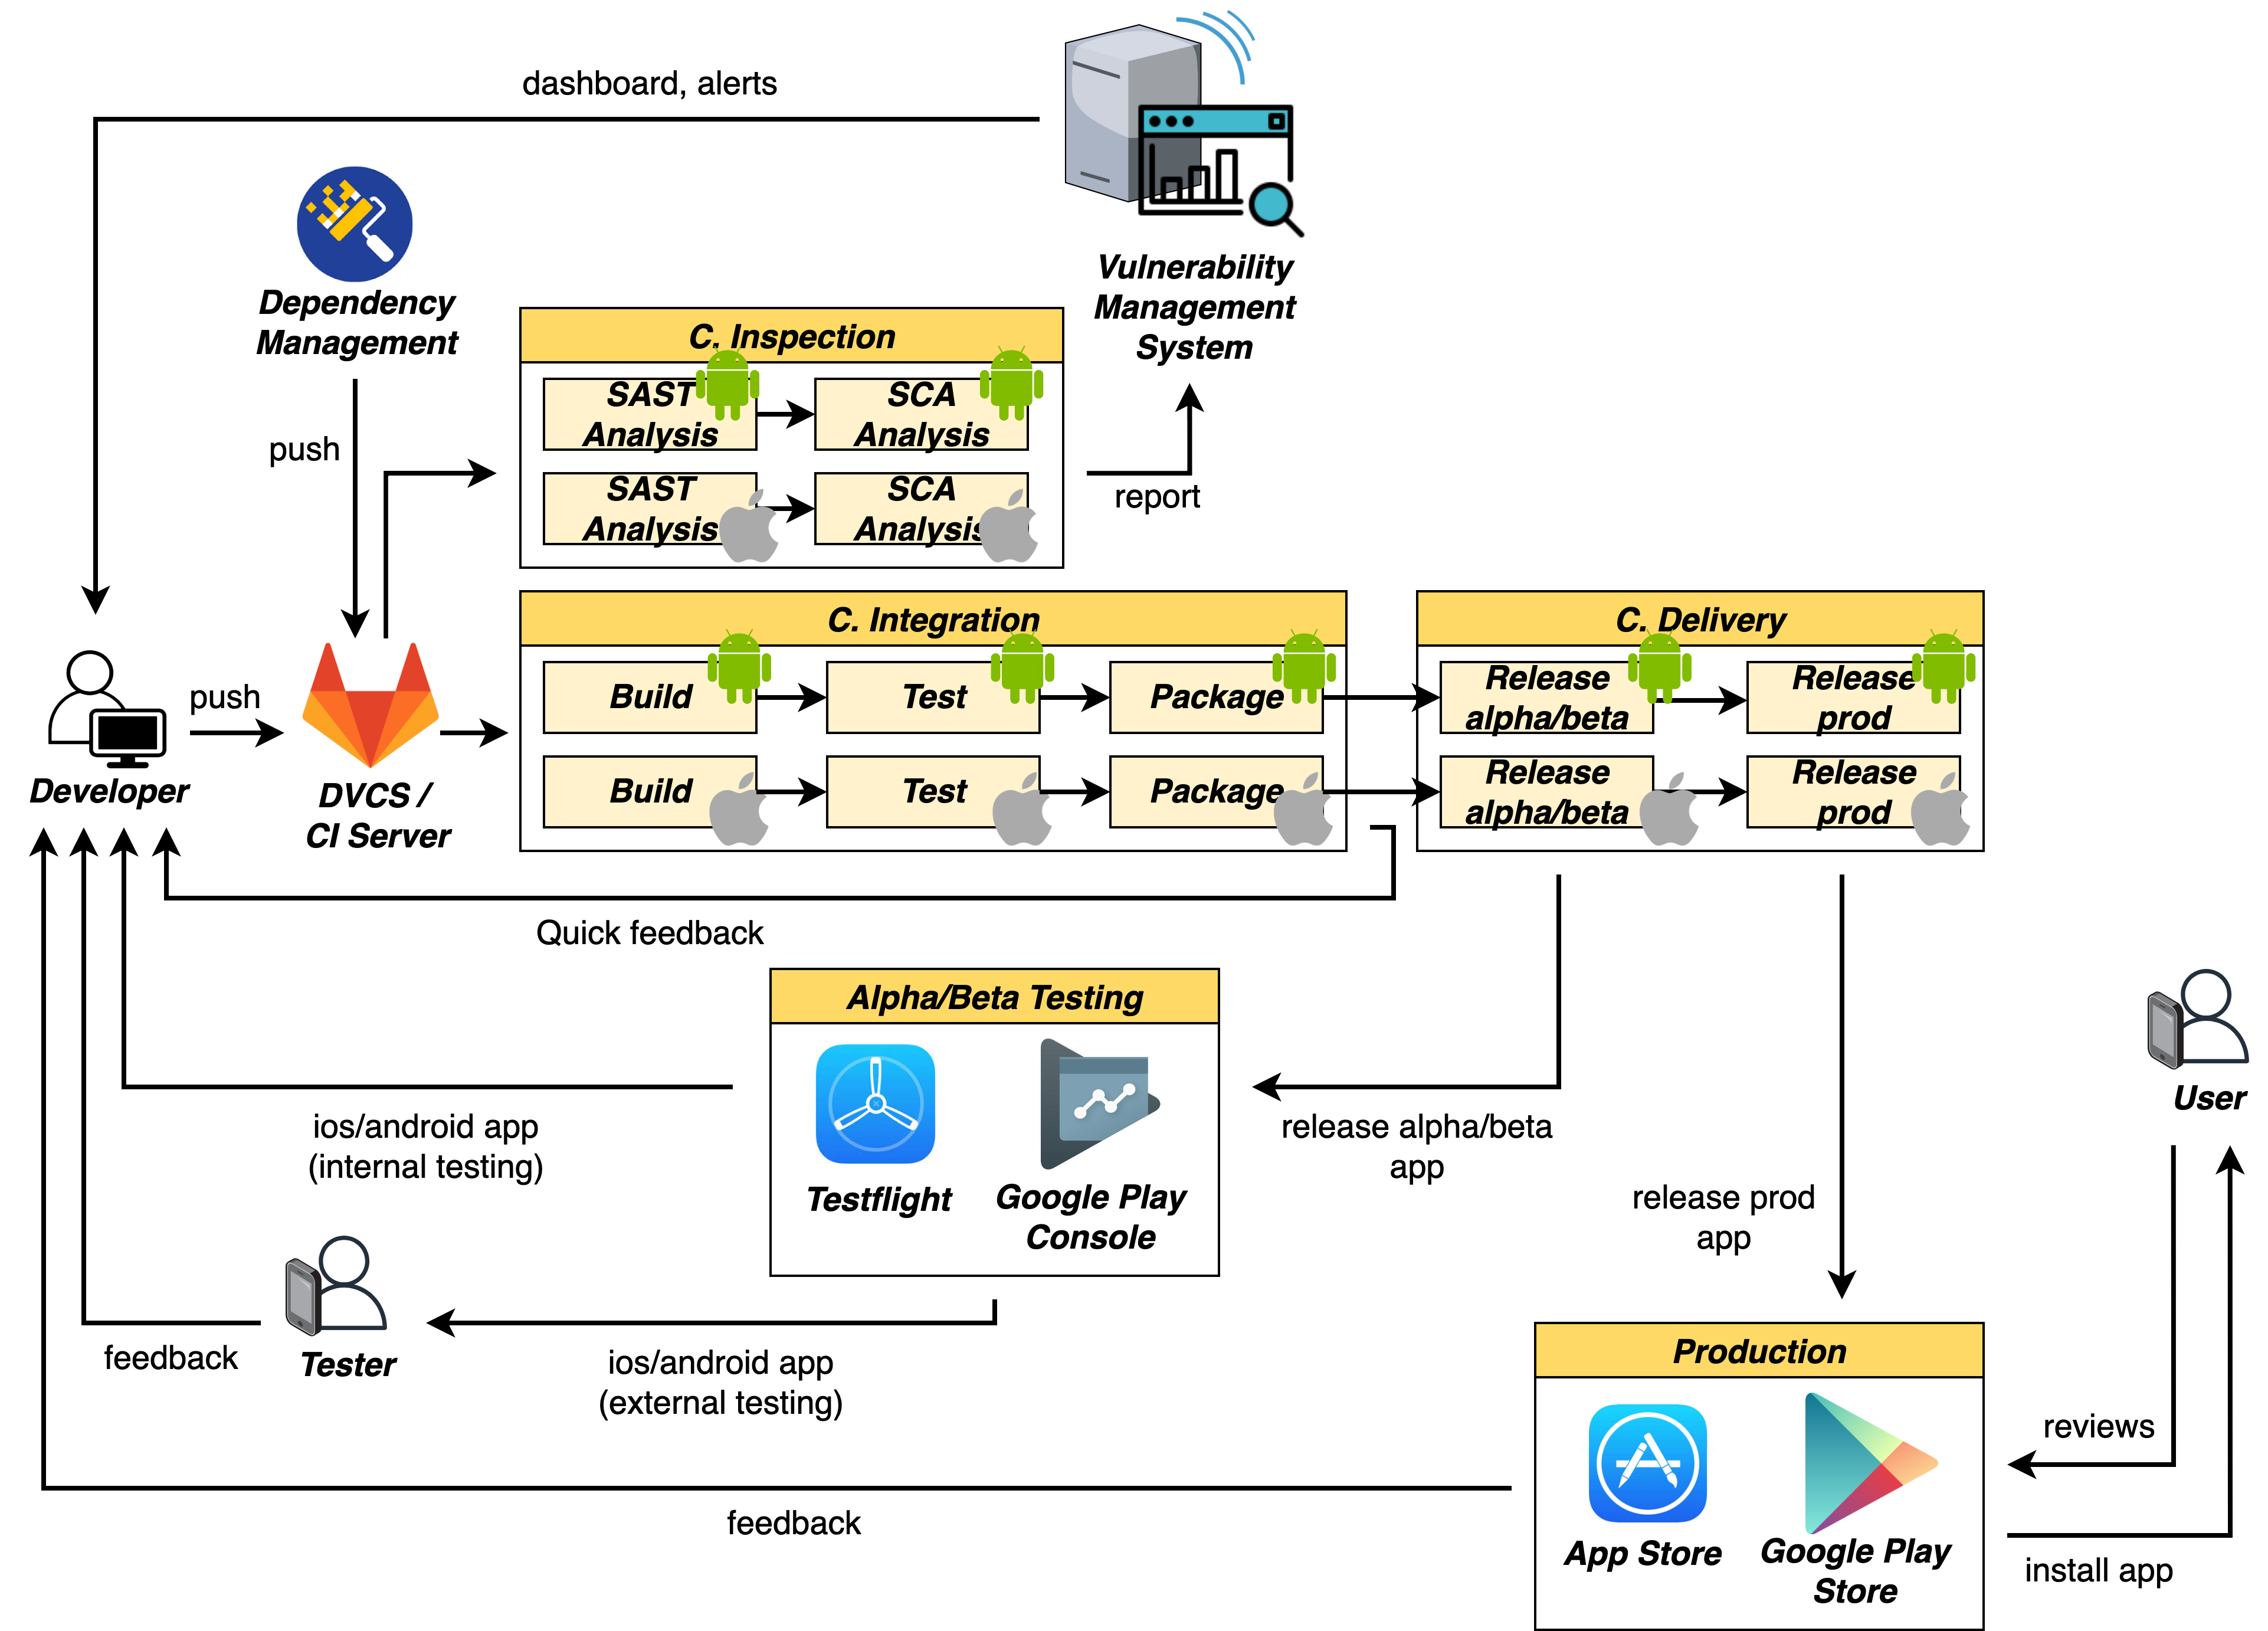
\includegraphics[width=0.85\textwidth]{img/full-cicd.png}
    \end{figure}

\end{frame}